\documentclass[11pt,a4paper]{article}
\usepackage{natbib}
\usepackage{a4wide}
\usepackage{graphicx}
\usepackage{lmodern}
\usepackage{fullpage}

\pagestyle{plain}
\title{\textbf{Investigation into the causes of the impact Under 13 funding}}
\author{Greig Russell}
		\date{\today}

\bibliographystyle{apalike}

\usepackage{graphicx}
\begin{document}
\maketitle

\pagebreak

\tableofcontents

\pagebreak
\pagebreak

\listoffigures

\pagebreak

\section{Executive summary}

\section{Introduction}
On the 1st July 2015 the government implemented its election promise to make care free for all children aged 6-12 years who were registered with a Primary Healthcare Organisation.\\

For primary health care providers, the focus was about getting adequate compensation to offset any income loss. Within the secondary care environment, little comment was heard. This funding change was only seen as impacting primary care and even then in a marginal sense.\\

What happened was totally unexpected. By chance the commencement date coincided with a nasty influenza season leading to record numbers attending the Emergency Departments and Urgent Care clinics. These traditionally last six to eight weeks before settling. Only it did not not.

\begin{figure}[htp]
\centering
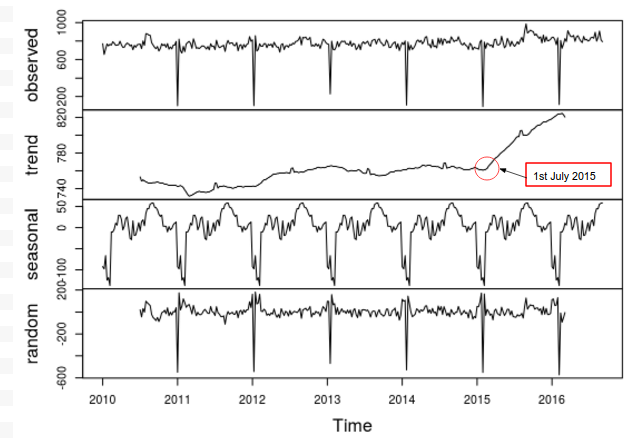
\includegraphics[scale=0.50]{TS_ED.png}
\caption{Time series analysis splitting from all Emergency Department presentations, the changing trends for utilisation from the underlying seasonal patterns.}
\label{Time series analysis of Emergency Department presentations}
\end{figure}

This change in utilisation patterns is even more marked for those who have used the department for two or three times within the same year.

\begin{figure}[htp]
\centering
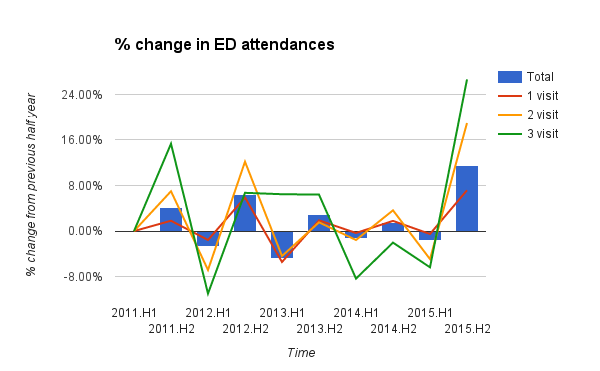
\includegraphics[scale=0.50]{Fchange.png}
\caption{Changes in ED utilisation in H2 2015, especially for rates of second and third time utilisation within the quarter}
\label{Changes in Ed utilisation}
\end{figure}

Yet within General Practice itself, little sustained change in utilisation by the 6-12 years age group was noted.

\begin{figure}[htp]
\centering
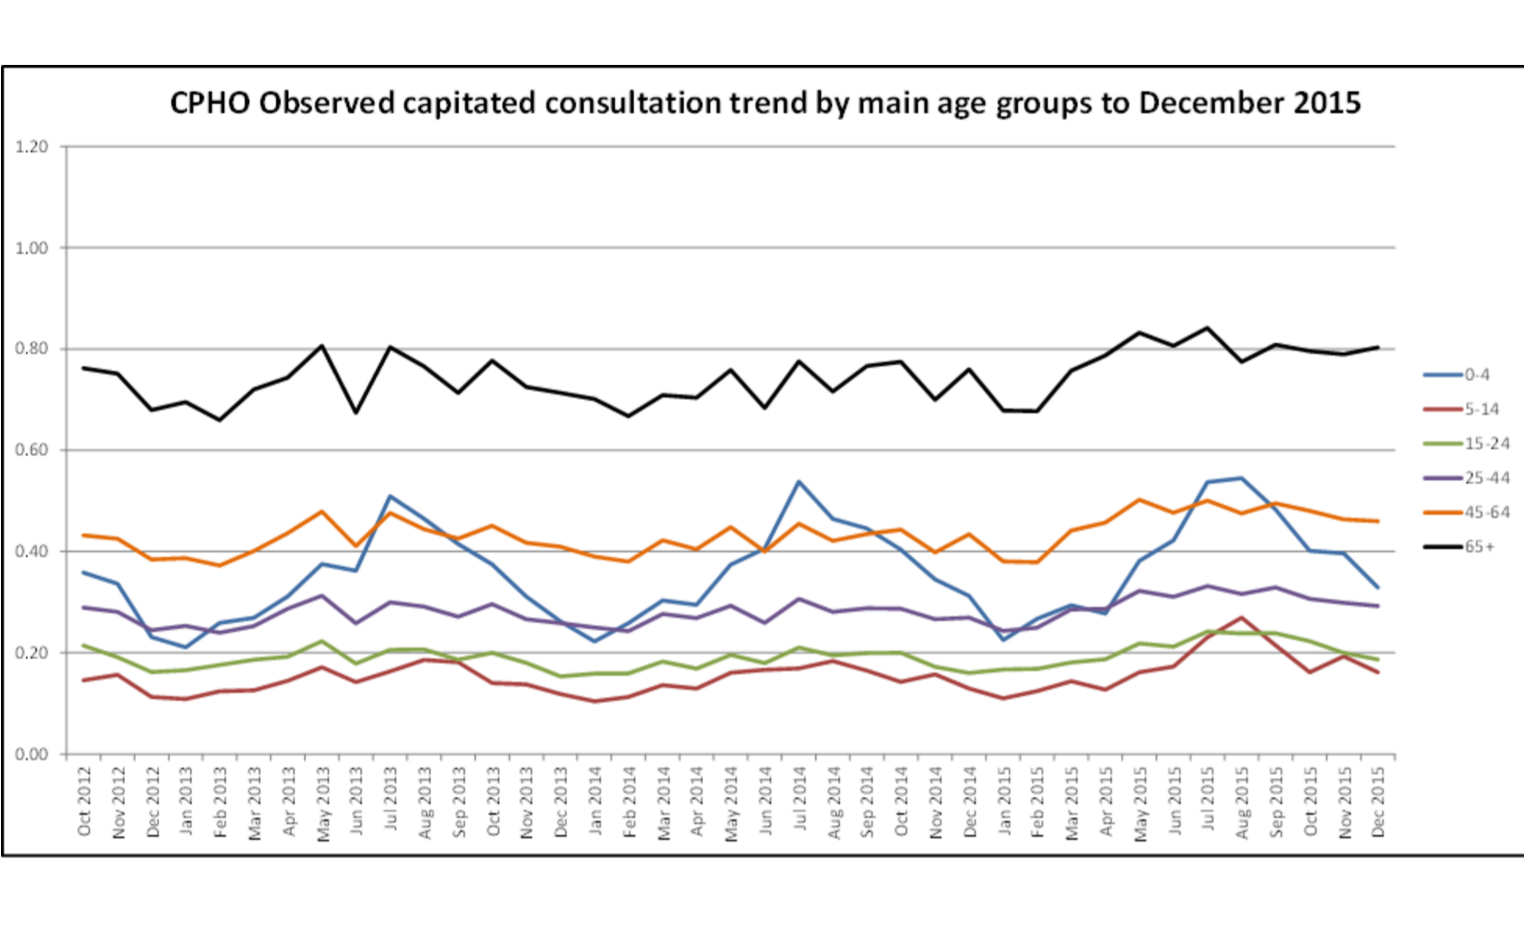
\includegraphics[scale=0.40]{U13one.png}
\caption{Stratified rates of GP consultations for Central PHO practices}
\label{Age stratified General Practice consultations}
\end{figure}

This change in utilisation has persisted ever since as the new normal.

\begin{figure}[htp]
\centering
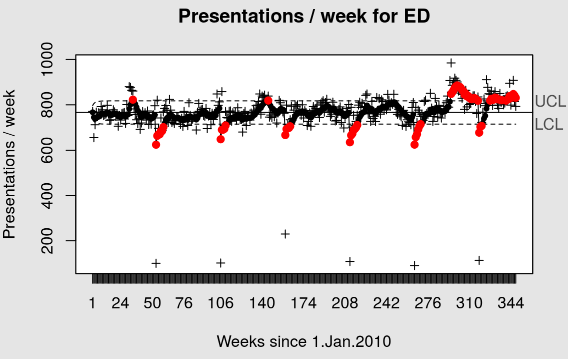
\includegraphics[scale=0.40]{EWMA_ED_pesentations.png}
\caption{EWMA chart of weekly ED presentations since 2010, with weeks put of control limits being displayed in red.}
\label{EWMA statistical process chart of ED presentations}
\end{figure}

and the projections for the future show growth continuing through until 2017, so creating a capacity crisis within the physical Emergency Department

\begin{figure}[htp]
\centering
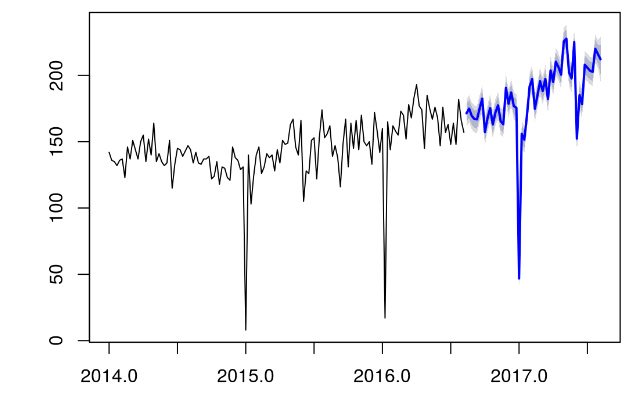
\includegraphics[scale=0.40]{HW_projections.png}
\caption{Projection for ED utilisation using a Holt-Winter's methodology.}
\label{Projections for ED utilisation through to 2017}
\end{figure}

 This unexpected result was contrary to what was envisaged by the  New Zealand Primary Health Care Strategy \citep{king2001primary}. In 2001, the Primary Health Care strategy was released by the then Minister of Health, Annette King \citep{king2001primary}. The aim of this new strategy was to transform the health care landscape within primary care, but with a transformation that reflected the priorities and perspectives of the newly elected Labour Government.\\

Minister King inherited a health system that had been through a series of changes, but which had remained the same from a patient perspective for many decades. Until the early 1990s, the New Zealand primary care system had been one of a state subsidy based on a fee for service by a doctor \citep{gauld2006new}. With the neo-conservative health reforms of the early 1990s the split between funders and the providers of care was introduced, along with increased competition between providers as part of a drive for achieving the economic efficiency inherent within the true free market. General Practitioners were allowed to form Independent Practitioner Associations (IPAs) so as to form groups of sufficient size, so that primary care providers could participate effectively in a competitive health care model. These IPAs continued to be predominantly GP led and, as organisations, they remained focused on protecting their General Practitioner members from any negative impacts of the neoliberal health reforms \citep{malcolm1999new}. Some IPAs achieved successes through profit sharing arrangements with the new funding bodies, but essentially from a patient perspective it was business as it had always been. The Government funding of primary care provided less than 10\% of income during practice in this era. This percentage of practice income provided by the state to subsidise patient fees and ease access to community based health care was reduced each year. As the rate of inflation was greater than the rate by which the subsidy increased, the subsidy became an increasingly smaller component of practice income. Even this limited subsidy applied only if the doctor saw the patient and did not apply if the patient saw the practice nurse. This activity based funding system led to absurdities through valueless over servicing. \\    

The Primary Health Care Strategy wanted to achieve a more fundamental reform of primary care and had broader aims \citep{king2001primary}. Under the strategy, health care was to be about the health of entire populations and focused on providing preventive health care delivered by multidisciplinary teams. The funding of primary care was to be on a capitation basis where subsidies to practices were on a fixed income per annum per enrolled patient and not on an activity basis. It was in a practice's financial interest to spread consultations across all team members as this improved profitability by increasing the number of patients the practice could enrol. Only by focusing on preventive health care could the required reduction in consultation rate per patient be achieved for the practice to live within its means. \\

The shift to capitation-based funding also removed the funding barrier to non-medical providers participating in health care provision. Indeed, a fixed income should have encouraged practices to use cheaper nurses to provide patient care than more expensive doctors whenever possible. Indeed, it was imagined that nurses could open their own practices without doctors. Envisaged in the strategy, was that all professional groups could now contribute to overall community health outcomes, with each team member working at the top of his or her scope of practice. \\

Driving the adoption and success of the new strategy was an increase in overall health funding of \$500 million per year from 2002-2008 \citep{gauld2006new}. Increased demand for health care, especially in areas of deprivation, was to have been driven by this dramatic increase in funding \citep{king2001primary}. From the perspective of "supply and demand" microeconomic theory, the Primary Health Care Strategy aimed to establish a local free marketplace, with funding to enable all patients to participate as they sought the best deal from multiple suppliers or practices. Patient demand was to drive primary health care to the optimal allocative efficiency of resources to meet their health care needs. It was envisaged, moreover, that the behavior of the primary health care market in a given locality would be regulated automatically by the 'invisible hand' or inherently self-regulating nature of a free market. In this situation, the focus of the Government was to be on ensuring participation of those from areas of deprivation and poverty. \\ 

The challenge in this field of study, has been how to evaluate the actual impacts of the strategy on society and the health system. As without an understanding of how the strategy impact utilisation of primary care, there will not be an understanding of how increasing funding for one group to receive easier access to community case lead to a dramatic rise in utilisation of the emergency department.

\section{Literature review}
Studies considering the impacts of the Primary Health Care Strategy have produced conflicting responses to date. \citet{hefford2005reducing}, examined the strategy's results 15 months after implementation. The authors described the development of performance indicators to allow any effects of the strategy's introduction to be tracked, especially with regards to correcting inequities. The study described  how this increased funding was cumulatively supplemented for those living in areas of high social deprivation by an additional 20\% per enrolled patient in a practice, and by another 20\% for every self-identified Maori or Pacific Islander, who enrolled (p. 14) in the practice \citep{hefford2005reducing}. One clear intention of the strategy was to shift these groups of patients from being financially undesirable to being financially highly desirable. This shift would attract providers to areas of high need and hence correct long-standing health inequities to exploit this new opportunity. If the total enrolled population of ethnic minorities and those who lived in areas of high social deprivation was above 50\% of the locality's enrolled population then further funds were provided to every practice in the locality. \citet{hefford2005reducing}, found that those most in need had enrolled in greater numbers than the general population. The overall level of funding that these ethnic minorities and those patients from socially deprived areas  received was 25-60\% higher under the strategy than under the previous funding formula. The authors argued that this reduction in cost for these previously undesirable patients, and their observed greater uptake will lead to improved health outcomes. The authors described overseas studies which found this exact effect.\\

\citet{howell2005restructuring}, was less optimistic than Hefford. She argued that the strategy is the adoption of an insurance model where the individual practice in effect becomes an insurance agency, where the capitation is a premium that pays for a fixed quota of care. For Howell, once the quota of care is exceeded by the patient, the risk of the financial cost of ill health is transferred to the practice. She identified two groups of patients who will use excess care as compared their capitated funding and so create financial risk for the practice. The practice will then (probably) mitigate that chance by passing the costs of excess use back to the patient through fee rises to all patients.\\

Her first group was the worried well, who may seek more care than their capitation funding allowance, attracted by the reduction in prices. The second group who might care above their capitation funding was those patients with a chronic illness, especially those with multiple comorbidities, attracted by lower prices to get necessary care. The amount of care sought again is in excess of the capitated allowance.\\  

To manage these financial risks the patients fees would rise, especially within a small cohort of patients, such as the 1-3 doctor practice. As spreading the risk of the few across a large cohort of patients would powerfully mitigate these potential risks, Howell argued that any fee rises have adverse effects on the effectiveness of the Primary Health Care Strategy. The affluent, given their greater weekly income, would experience against a background of higher disposable income as only a relatively small reduction in fees affordability. Any fee rise would have a disproportionate effect for poorer people, though, given their initial lower weekly income, so once again fees would act as a barrier to those seeking appropriate care. These increasing costs would act as a disincentive particularly for the preventative care of those with chronic illness and need more frequent attendances to achieve maximal outcomes.  \citet{howell2005restructuring} described how, in order to prevent fees rising, the then Labour government would have had to restrict the historical right for General Practice to control their charges independent of external regulation and change the historical fundamental business model of General Practice away from individual ownership to a collective.  The Labour government was unable to achieve either change.  \\

For \citet{howell2005restructuring}, then, after an initial period of readjustment the patient costs would rise, and the focus of General Practice would remain on those who can afford to be sick. Howell argued for the adoption of an actual insurance model. If such a model was adopted, then the financial risk of chronic illness and the ability to manage locality derived utilisation patterns would be carried by a much larger group of patients and providers than was achieved under the Primary Health Care Strategy by 2005. This would reduce the drivers towards fee increases and its associated distortions to the system.\\

Depressingly, more recent evidence seems to support Howell's pessimism rather than Hefford's optimism when considering the potential of the strategy to achieve its goals of reducing health inequity within the population by providing equality of access. \citet{jatrana2009primary}, described the impact of the strategy on primary care utilisation. Those with the greatest number of current comorbidities, current smokers, those who felt their health was poor, those who had limited education and those who came from the most significant levels of social deprivation - were all likely to delay seeking medical review and were much more liable to delay filling a prescription.  As an example, consumers who were in the NZ Index of Deprivation of 5 or higher were 18.01 times more likely to delay seeking medical review as compared to the lowest group in the NZiDep and 24.47 times more likely to delay filling any prescription. \citet{cumming2008reforming}, considered  that although the Labour government was injecting considerable extra funding each year under the strategy, this increase of financing was not passed on as fee reductions.  In fact, by 2005, patient charges, rose on average for adults by 18\% (or \$4.30 / consultation). In practices with the higher levels of social deprivation and large concentrations of ethnically disadvantaged patients, the fees dropped by 20\% (or \$4.40 / consultation) for adults. This reduction represented a small percentage drop in overall household weekly income, militating against its effectiveness in reducing health equity.  The authors described how the most significant impact of the rise in health funding during the implementation of the strategy was the 58\% increase in GP income from \$97,220 to \$153,886. This growth in practitioner income together with overall patient fee rises supports Howell's opinion that the GPs continued to manage income from fees as they had done previously, without adopting a managed risk approach, and that they continued to use fees to manage fiscal risk from chronic illness. \\

\citet{howell2005restructuring} prediction was that fees would again become the primary economic driver for the financial stability of practices. Driven by the ageing  population, there would an associated projected rise in the number of patients with chronic illnesses and multiple comorbidities that would lead to an increased  average utilisation rate greater than that provided under the capitation funding rates. The increased government funding provided through the initial roll out of the Primary Health Care Strategy would have offset the impact of increased utilisation on practice income. After the annual growth in funding ceased then the percentage of income from capitation would have to fall as a percentage of total practice revenue, and a rise in the fees derived income would be needed to offset that reduction in the face of rising utilisation.\\

\section{Methodology}
This study was set in the geographically isolated city of Palmerston North with its population of ~78,000 people and considers the effectively closed system from both a health care provision as well as an economic perspective.\\

\begin{figure}[htp]
\centering
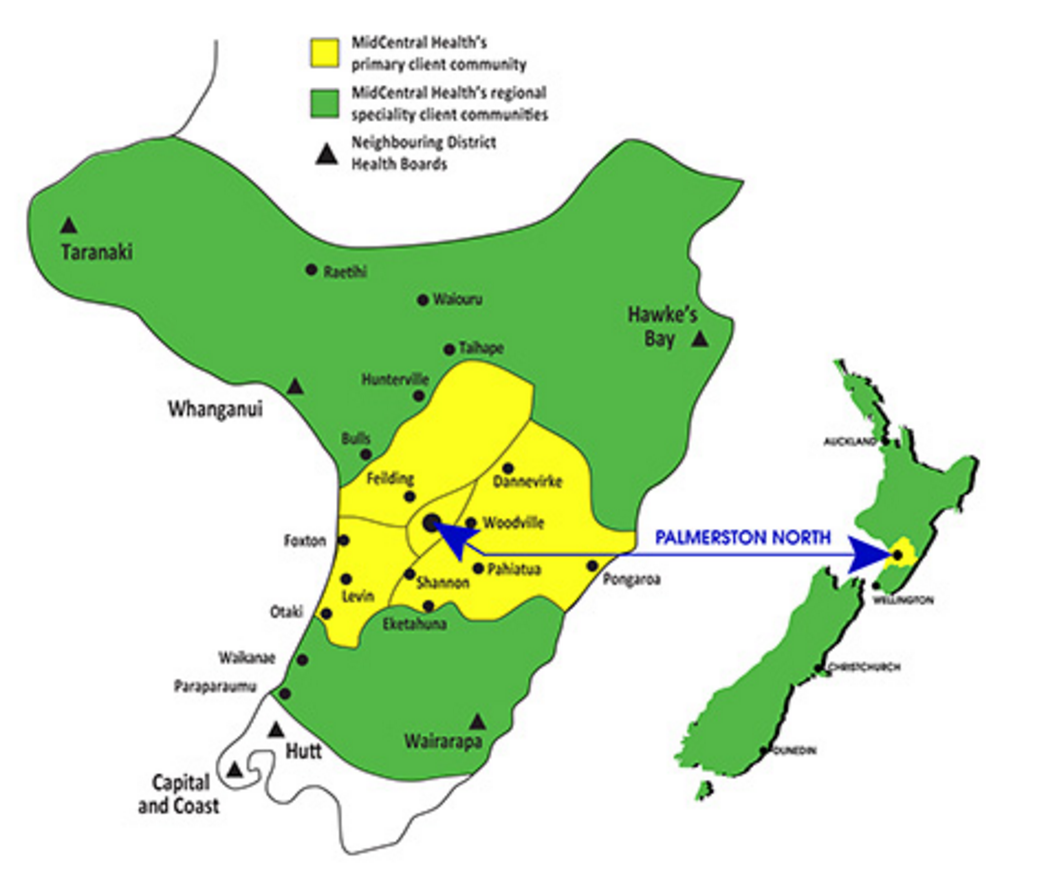
\includegraphics[scale=0.5]{fig1.jpg}
\caption{The location in New Zealand and the total area of responsibility for MidCentral DHB}
\label{MidCentral District Health Board}
\end{figure}

Conveniently Palmerston North is laid out as a rectangle, with deprivation believed to lie in equally distinct quadrants, although this was not later confirmed.\\

\begin{figure}[htp]
\centering

\includegraphics[scale=0.20]{fig2.png}
\caption{The traditional view of the economic layout of Palmerston North. The poorest sector is the top left quadrant, the richest in the bottom right. In between lie the middle classes.}
\label{Traditional view of the spatial economics of Palmerston North City}
\end{figure}

The introduction of the primary care strategy led to the disestablishment of the previous General Practice governance structures. This in turn resulted in the loss of all data prior to the disestablishment and this was an unforeseen complication in this study. On review of the options for historical information, the assumption was made that commercial organisations, including medical practices, generate business by advertising. As part of advertising, the address is also supplied along with the nature of the business. Telephone directories are public information, and are held in the local public library. These served as the basis for the geographic data set used in this study.\\

The data collected was simply a table of names of practitioners, the address they gave in the telephone directory of the year and the nature of their practice (solo vs. small group practice vs. large group practice with over five practitioners at a single location,  General practice vs. Urgent care vs. Specialist Care). Only the  medical practices listed in the specialist medical practitioner section of the telephone directory were included. The current government is encouraging the formation of large integrated family health centres. As a byproduct of this further development, the intended location and nature of practices is also known in 2016.\\

Difficulties with using the telephone directory as a data source were immediately apparent, including, for example, occurrences such as a failure to update addresses when practitioners moved to new premises. It was, in addition,  impossible to determine whether there were omissions from the directory. Some group practices only list their medical director, not all medical and nursing staff employed there. As a consequence, the contribution of such practices to the overall provision of health care will be under estimated.  After discussion, it was decided to proceed with the limitations in the data set as no better data set was available.  \\

Clearly there are many interdependent factors in any given market that will impact on economic activity by retailers, independent of macroeconomic policy for niche markets like health. A classic example is the 2009 global financial crisis that affected all business including health. To control for these local or global effects on the whole local market, retail alcohol was chosen.  This group was selected as they provide services of similar cost, with similar hours of operation but are not subsidised by central government. Only those hotels, retail alcohol outlets and bars in the relevant sections of business section or "Yellow pages" were considered to be part of this control group. There were similar limitations in the data with regards to this group as there were for medical practitioners.\\

The analysis method comprised of two phases. The first was to use GIS to plot the changes in the geographic distribution of General Practices in Palmerston North city from 2002 - 2016. The second phase was to try to understand the distribution and changes over time against controls or alternative possible hypotheses. \\

Analysis was carried out using two tools. The network analysis and Heat maps were completed using Google Fusion tables, while the statistical analysis and visualisation of the results were completed using Google Sheets. The Graphic Information System analysis was completed using Google maps. All data was held in a secure data repository that is compliant with FISMA, ISO 27001, ISAE 16/3402 and HIPAA international standards for health data storage. In dealing mathematically  with the inherent issues in this data set, it was treated as a sample not a population. This adjustment partially compensated for the data quality issues. Classical microeconomic theory and game theory was used to consider the results of the GIS study from an economic perspective. \\

Local ethical approval for this study was obtained via the MidCentral Health Clinical Board. The Clinical Board is responsible for all local Health research undertaken within the District Health Board, including primary care.  Regional approval from the Central Health \& Disability Ethics Committee (HDEC) was not required as this study was deemed to be  a low or minimal risk. \\

In economics, Game Theory is used to explain or develop a winning economic strategy. All businesses that adopt this optimal strategy flourish or at least survive while those that do not inevitably perish. A strategy can focus on the range of goods or access to the market. In health markets like primary care provision, then the range of products and internal business model is similar to all providers, so the  only variable that can change is the market's ability to access that provider \citep{dinar2008game}. \\

To demonstrate this concept, the most frequently used example describes two ice cream vendors on a beach. The first sets up in the middle of the beach and gets unique access to 100\% of the market. With the arrival of the second, the profit-maximising position for them both on the beach is for one to be at 25\% along the beach and the other at 75\%. The reality is both will be found in the middle, with both ice creams vendors beside one another selling the same goods at the same price. Game theory predicts this because if one vendor suddenly moves to the middle of the beach, then they will control 75\% of the market, a considerable gain. The other vendor, who stayed still, will only control the other 25\% position. The profit maximising position may therefore create the most profit, but also promotes the most risk. If both move to the middle, neither can lose a share of the market to the other and so this is the position where neither can lose from the actions of any one else, and no party consistently gains by moving away from it. The middle position, which minimises the risks to all players, or the position of no regrets is called the Nash Equilibrium. In a stable, mature market, the geographic position of business clusters is described as  the Nash Equilibrium between the economic forces under which the businesses operate. If two groups of businesses have similar Nash equilibrium positions as seen from geographic locations, then they operate under similar economic forces. If they are in different locations then the two sectors are reacting to various economic drivers. \\

Game theory has been applied to the development of health systems. \citep{dobson2004sustainable}, used the combination of game theory and social network analysis to understand the development of an integrated local mental health initiative. This study found that the outcome of the initiative for participants was driven by the social network in which decisions were made. The analysis was made by analogy to the famous game called the "Prisoner's dilemma", where the players get a moderate adverse outcome through cooperation, while one would receive a favourable outcome and the other a much worse through not cooperating. This study suggested that, by failing to consider how to optimise their position, the participants left themselves vulnerable to the worst case outcome. \\

\citet{tarrant2010continuity}, have used Game Theory to understand the drivers behind patient trust of primary care physicians and how that changes with time. There were difficulties previously in understanding engagement, whether long term relationships lead to the evolution of trust in primary care physicians and if so, the reason behind this development. The authors' use of Game Theory enabled them to describe the underlying "game" of the therapeutic relationship. They found that patients started from a position of the generic physician encounter based on a social construct of the generic physician consultation. Game theory predicts that by repeated individual encounters, mutual benefit from the relationship develops as both seek insurance against "the shadow of the future" \citep{tarrant2010continuity}. Each participant makes no assumption of each others motivation. Indeed ill health is the shadow for the patient while financial insecurity or clinical medico-legal risk  are drivers for the physician. Game theory predicts that even without any shared motivations the optimal position for both is the development of a long term relationship to address clinical problems.  This study is not testing Game Theory but is using Game Theory to understand a social phenomenon. \\

\citet{chapman2012using}, used Game Theory to investigate incentives for uptake of annual influenza vaccinations.  The study found that when the incentives reflected self-interest the older group of players got vaccinated while the younger group did not. When the incentives were changed to reflect outcome for the total community (a "get vaccinated to protect your grandmother" style approach) the new Nash equilibrium position reflected a group-optimal utilitarian position. This study again used Game Theory to understand clinical behaviour in the community. It also showed the use of Nash equilibrium to illustrate changes in the net position of a population of non-cooperating individuals. \\

Game theory is in one respect an emergent economic theory, yet it is also an established theory, with an increasing repertoire of useful applications in different situations. \\

\section{Results}
For Game theory to have any applicability in a GIS based study there has to be geographical movement of practice location. Locally individual practices are, however,  noted for their longevity of location. This study revealed that General Practitioner turnover was greater than perceived in Palmerston North, despite the prevailing perception being focused on difficulties of attraction not retention. 

\begin{figure}[htp]
\centering
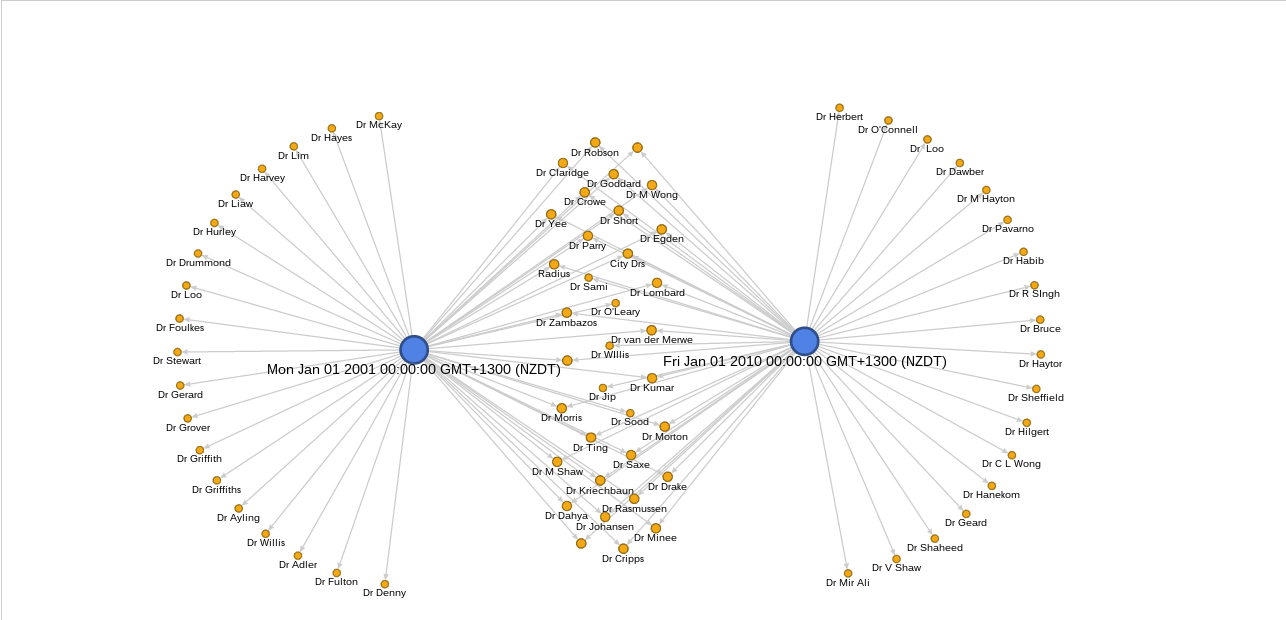
\includegraphics[scale=0.4]{fig3.png}
\caption{Network analysis showing General Practitioners present in 2002 and 2010, with the group in the middle present at both}
\label{General Practitioners present in 2002 and 2010}
\end{figure}

This turnover of practitioners was the mechanism of practitioner migration within Palmerston North. Where practitioners start new surgeries, they open them at new locations as compared to the surgeries that they replaced. The underlying basis for that decision is not conscious but does appear reactive to economic opportunities. This makes sense given the desire of any new business to be financially successful and the fact that new General Practitioners would not have any emotional or social attachment to the previous practice location.

\begin{figure}[htp]
\centering
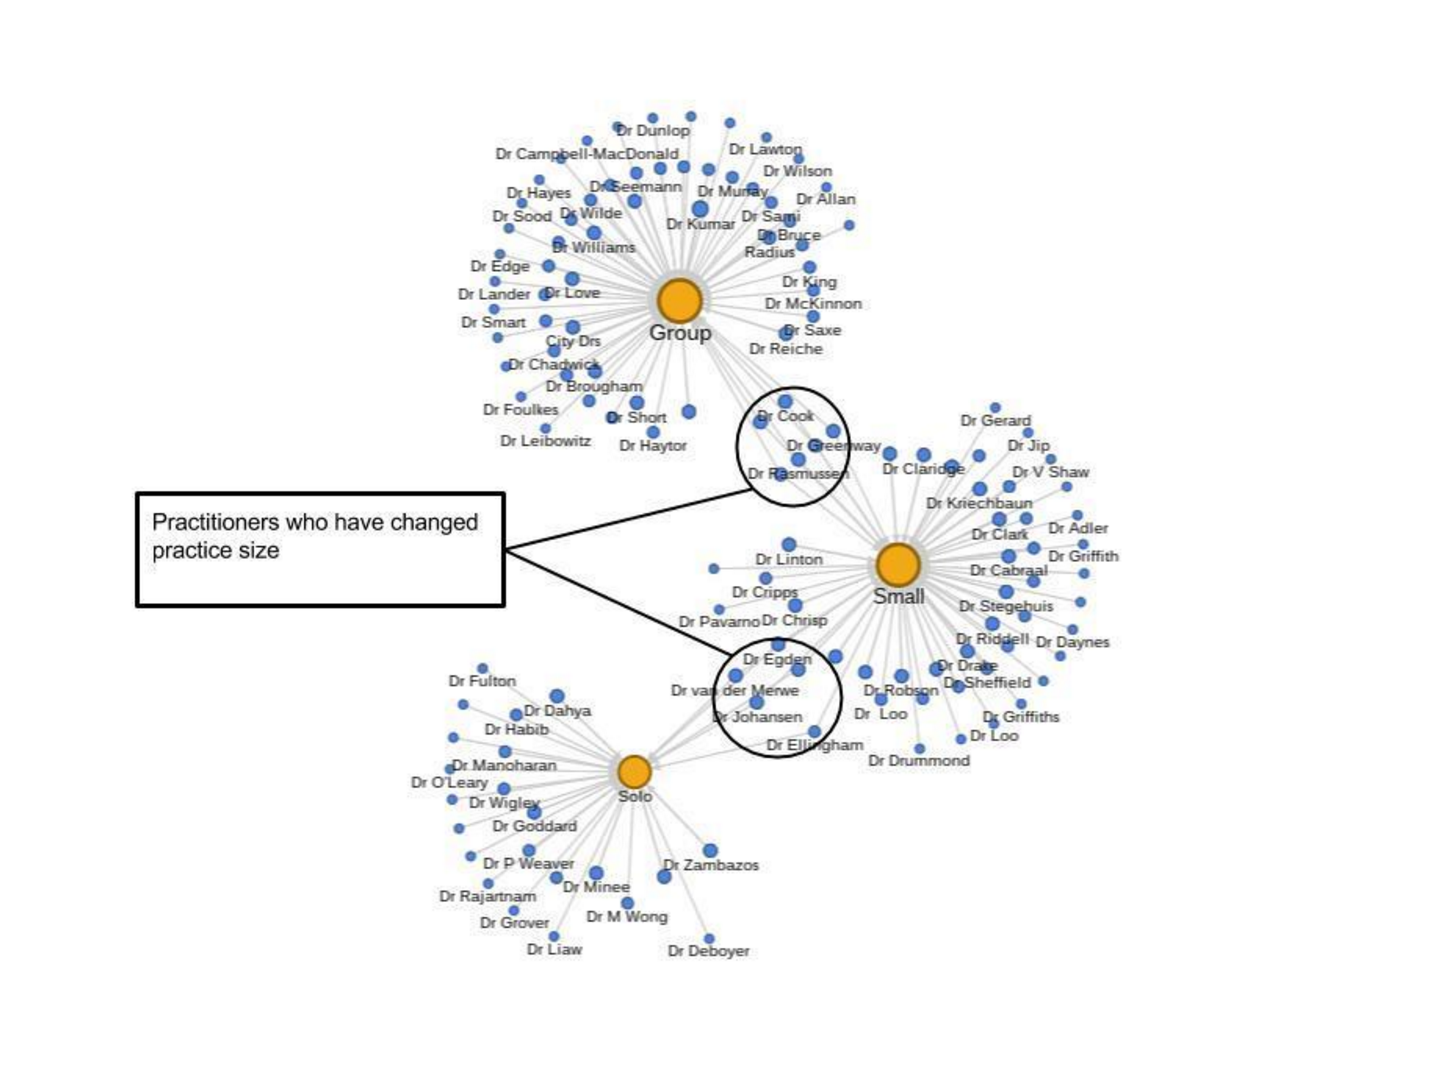
\includegraphics[scale=0.3]{fig4.png}
\caption{Social network analysis illustrating how few practitioners have moved after arrival}
\label{Movement of Practitioners between practices}
\end{figure}
 
\pagebreak

The raw results of the telephone directories and projections for 2016 revealed a far from stable population of practitioners: there is a diminishing population of providers in Palmerston North. There is a core group of practitioners who are pivotal to the stability of supply through their longevity in their practices with a wider group of assistants or transient practices supplementing primary health care delivery. That this group is starting to approach retirement is one of the drivers to establish integrated family health centres, so as to provide a vehicle for succession planning. This reduction in the number of practices is in contrast to the ambitions of the Primary Health Care strategy, one of the aims of which was to increase access through practitioner diversity.  \\

\begin{center}

\begin{tabular}{|l|l|l|l|}
\hline
	Provider type & 2001 & 2010 & 2016\\
\hline
	General Practitioners & 43 & 38 & 32\\
\hline
	Urgent Care & 8 & 10 & 9\\
\hline
	Specialist & 38 & 41 & 31\\
\hline
	Iwi & 0 & 3 & 3\\
\hline
\end{tabular}

\end{center}

Table 1: Summary of providers by type along with the retail controls. Where Iwi (Maori for local tribe) providers are marae (the Iwi's cultural and social forum) based General Practices. They have a different model of care focused on Maori values and priorities, and often located with other social services. Urgent Care Clinics are drop-in acute care clinics, which have a different non-health funding model to General Practice and are staffed by the different vocational scope of Urgent Care practitioners to General Practice. \\

As practitioners move into private practice, they are attracted to a specific practice configuration and this does not change this throughout their careers. Equally when practitioners move into private practice, they are attracted to a specific practice configuration and do not change this throughout their careers (see figure 5). \\

\begin{figure}[htp]
\centering
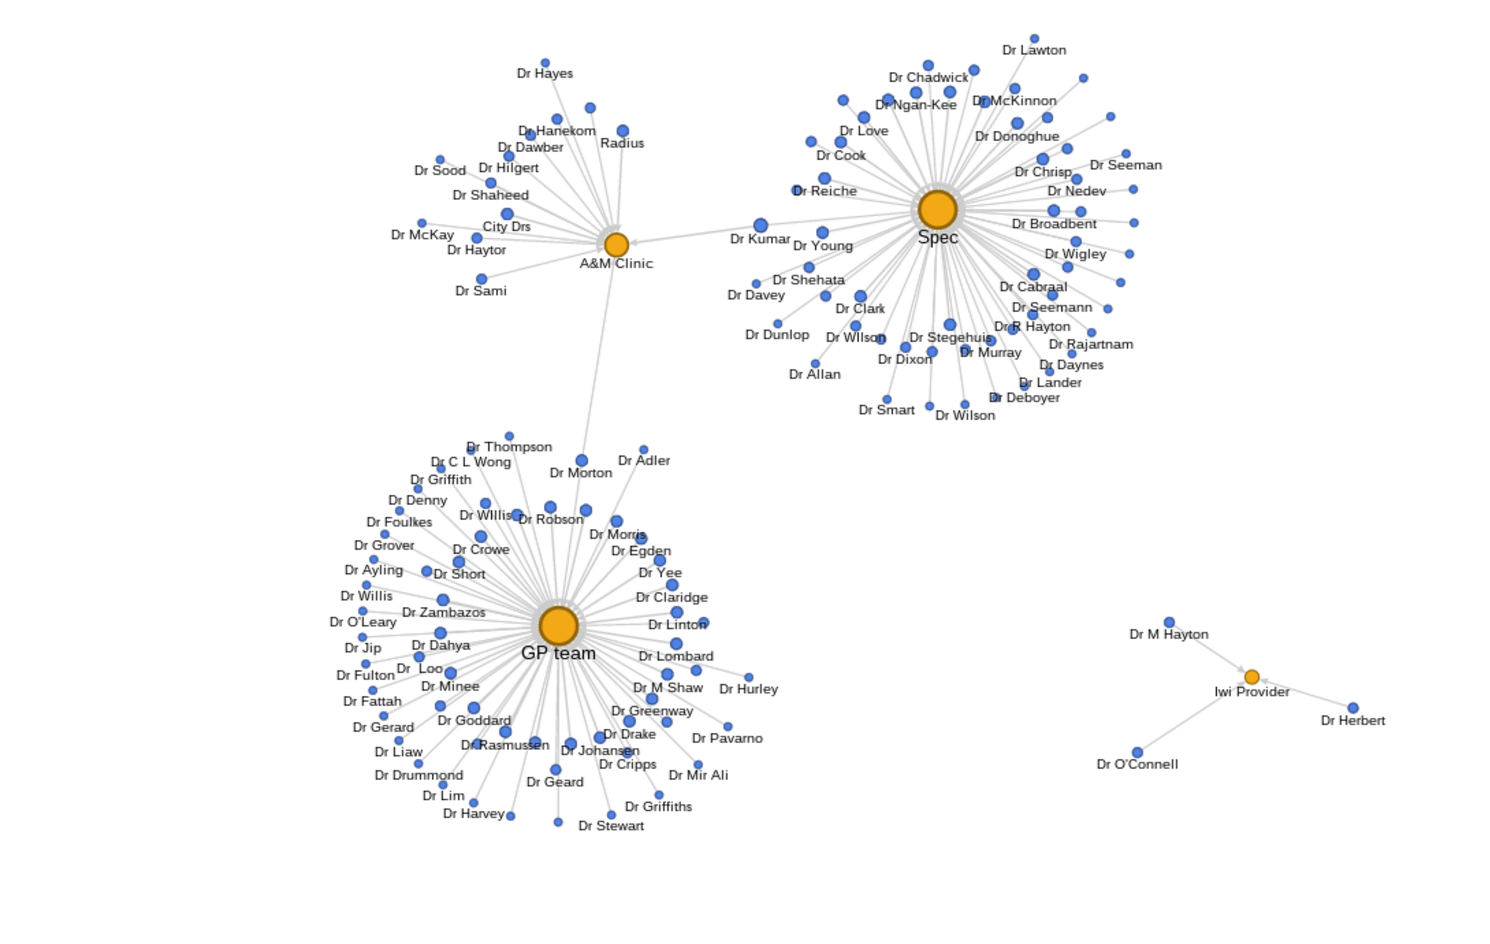
\includegraphics[scale=0.30]{fig5.png}
\caption{Social network graph of practitioner by practice type}
\label{Social network graph of practitioner by practice type}
\end{figure}

To consider geographic movements of General Practice over time, a series of heat maps was developed from the 2001, and 2016 data respectively.(see figures 6 \& 7).\\ 

\begin{figure}[htp]
\centering
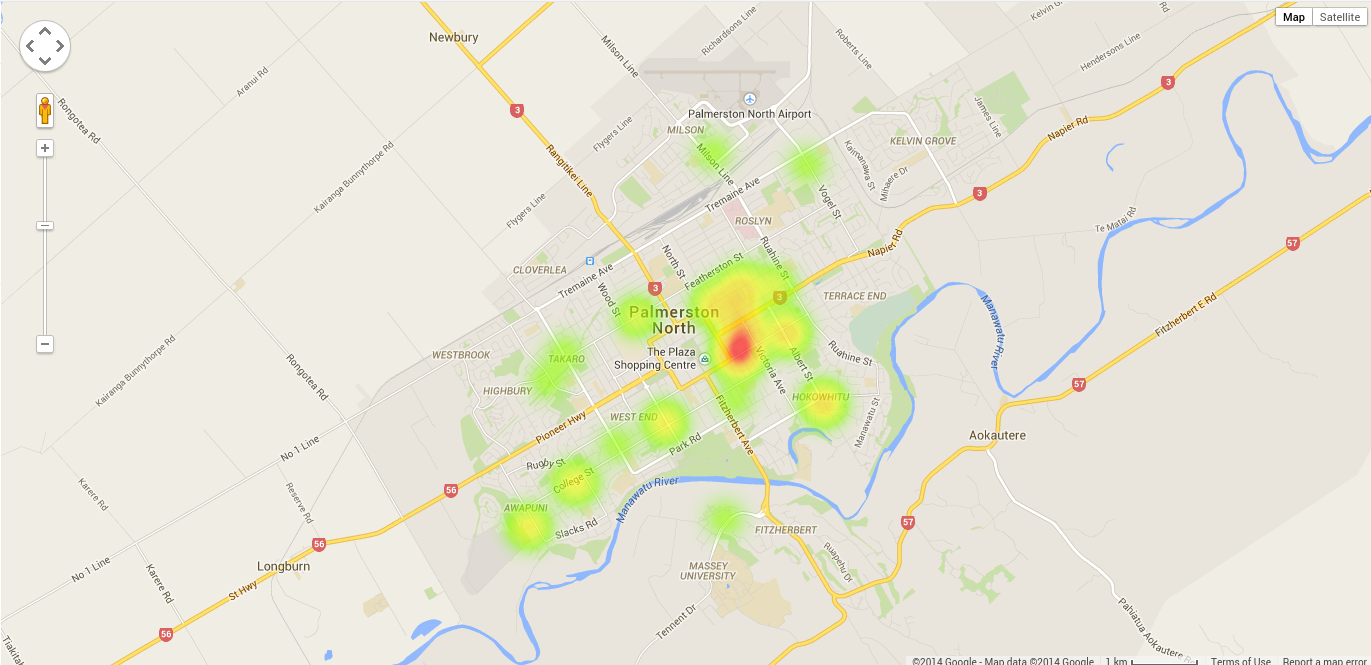
\includegraphics[scale=0.20]{fig6.png}
\caption{Heat map of the distribution of primary care provision within Palmerston North 2001. Please note that prior to the 2001 Primary Care Health Strategy there was even GP coverage of Palmerston North.}
\label{Heat map of practitioners 2001}
\end{figure}  

\begin{figure}[htp]
\centering
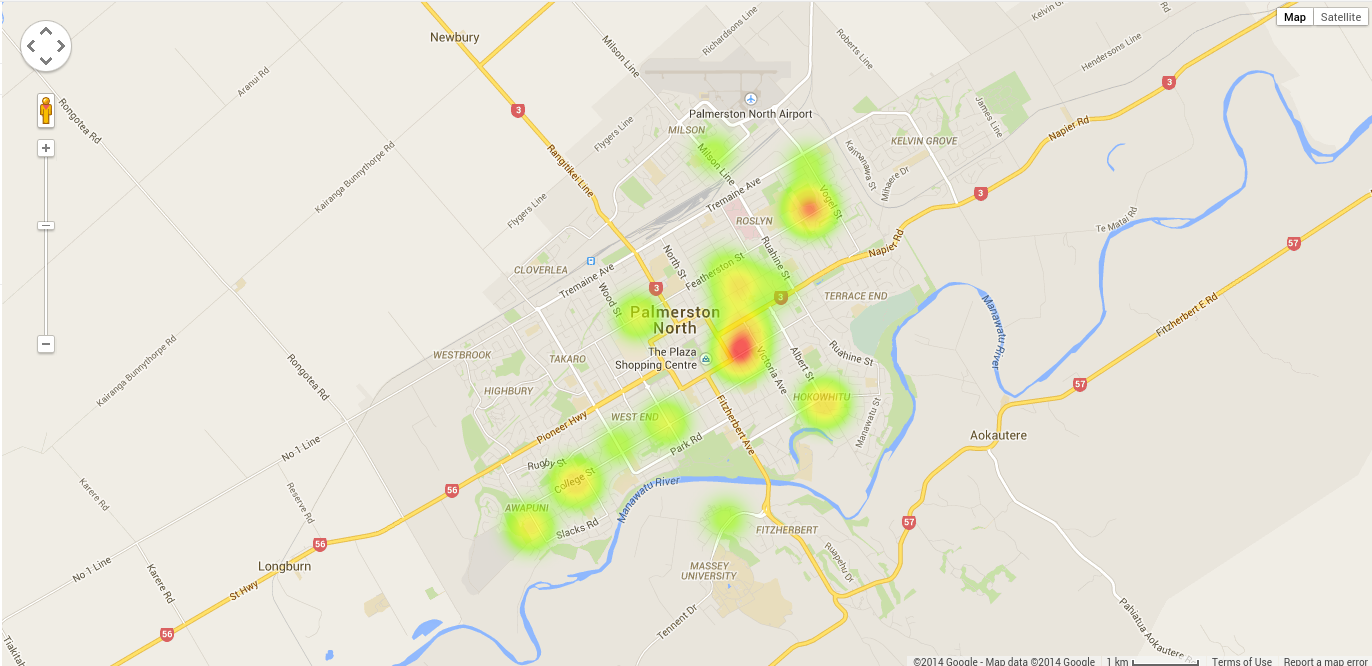
\includegraphics[scale=0.20]{fig7.png}
\caption{Heat map of the projected distribution of primary care provision within Palmerston North 2016}
\label{Heat map of the projected distribution of primary care provision within Palmerston North 2016}
\end{figure}

The distribution of primary care does not appear to match unmet clinical needs.  Consider the map of a sample of patients who presented to ED in 2015 without a current General Practitioner (see figure 8).\\

\begin{figure}[htp]
\centering

\includegraphics[scale=0.20]{fig8.png}
\caption{A sample of 1000 patients who attended Palmerston North Emergency Department,and did not have a GP in 2014}
\label{Distribution of patients with a General Practitioner}
\end{figure}

This distribution of General Practice providers is also quite different from services which aim to achieve equality of access across the town, such as the local bus service (see figure 9). There are, moreover no town planning barriers to the opening of new practices in the suburbs. \footnote{Palmerston North District Plan, R 10.8.1.4}  \\

\begin{figure}[htp]
\centering

\includegraphics[scale=0.2]{fig9.png}
\caption{Distribution of bus routes designed to maximise social equity and access by the public}
\label{Bus routes designed to maximise equity of access}
\end{figure}

\begin{figure}[htp]
\centering
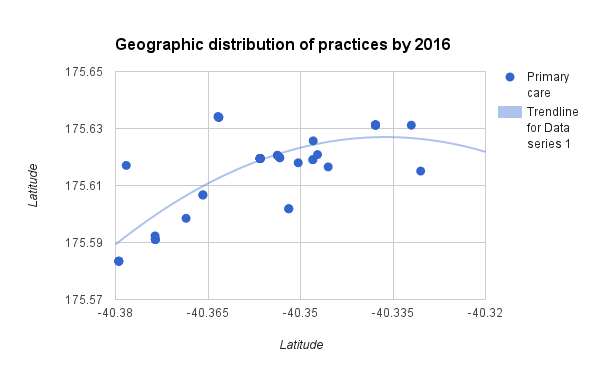
\includegraphics[scale=0.6]{Nash_GP_2016.png}
\caption{Scatterplot of General Practitioner location 2016, with a clear trend line present}
\label{Scatter plot of General Practitioner locations}
\end{figure}

Yet there is a clear pattern present underlying the distribution of General Practitioner by 2016 (see figure 10). Interestingly a similar pattern is seen when alcohol retail outlets are superimposed (see figure 11). \\

\begin{figure}[htp]
\centering
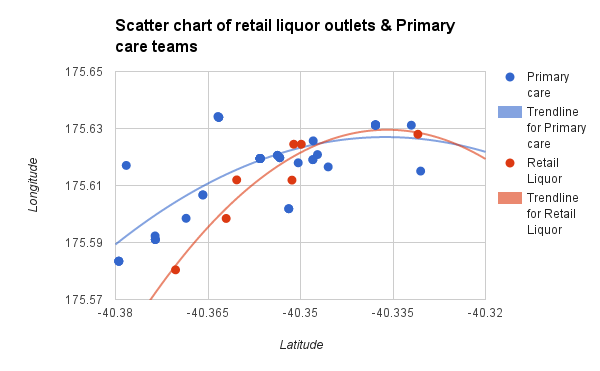
\includegraphics[scale=0.6]{Nash_GP_retail.png}
\caption{ Scattergram of both retail alcohol outlets and Primary Care providers in Palmerston North 2016}
\label{Geographic distribution of practices by 2016, with retail outlets overlaid}
\end{figure}

The distribution of both primary care and retail outlets appears to be maximised in the space between the two areas of affluence within Palmerston North (see figure 12).\\

\begin{figure}[htp]
\centering
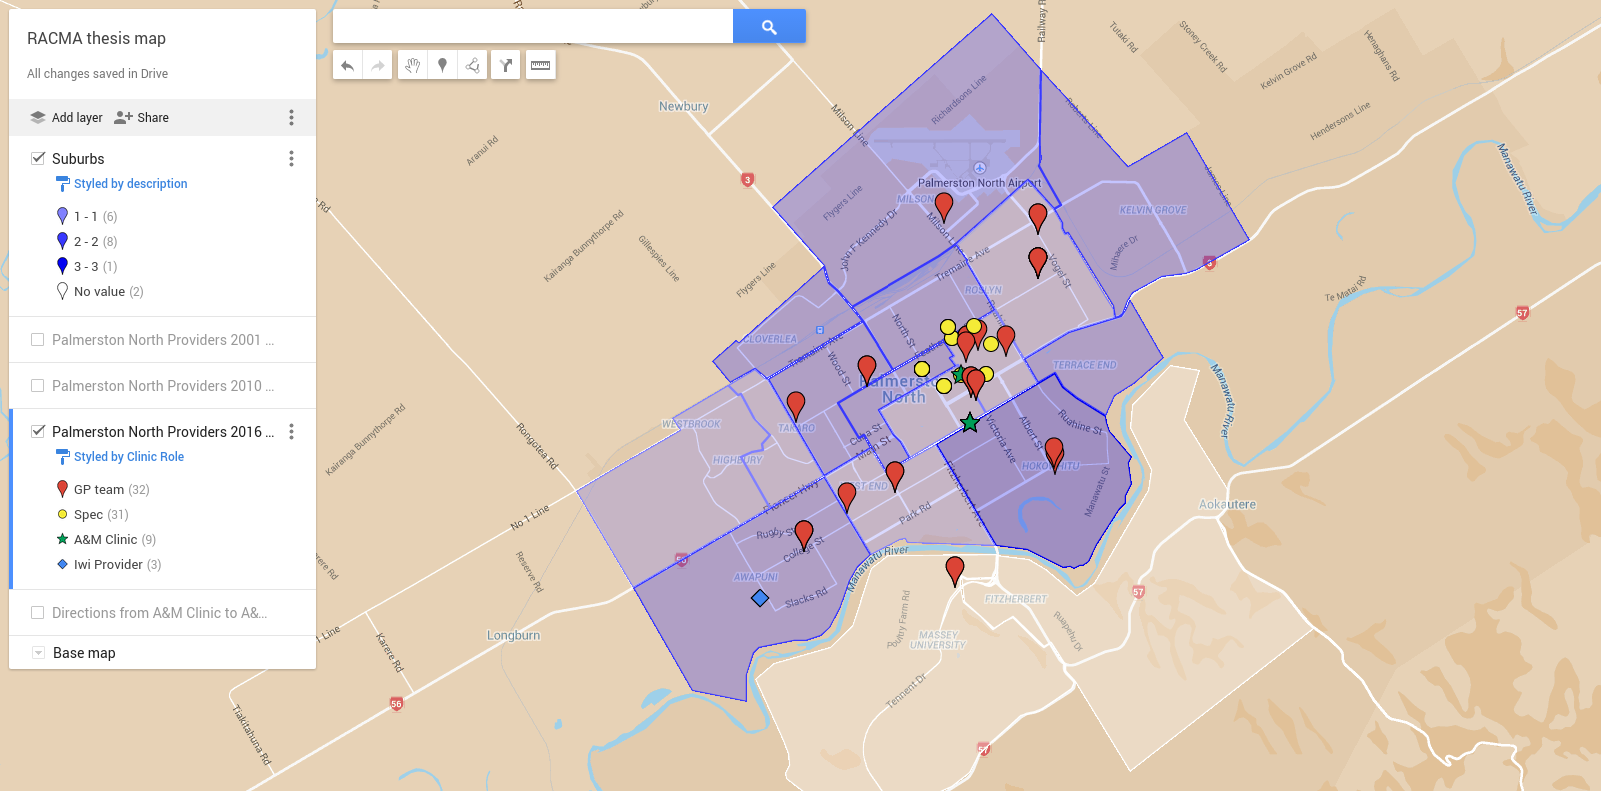
\includegraphics[scale=0.40]{fig12.png}
\caption{The distribution of both primary care and retail outlets appears to be maximised in the space between the two areas of affluence within Palmerston North.}
\label{Distribution of General Practitioners overlaid on suburb's social deprivation}
\end{figure}

\pagebreak

In summary, the use of Game Theory to analyse the results of GIS data enables an understanding of the microeconomic forces consequent to the changes in the macroeconomic policy. In this instance, Game theory analysis supports a proof by abduction that;

\begin{enumerate}
\item The location of primary care and retail outlets in Palmerston North are on almost identical geographical arcs.
\item The location of these arcs is equi-distant between areas of maximal disposable income.
\item Game Theory predicts this equivalence if both are driven by equivalent economic drivers.
\item The distribution of providers is not associated with unmet community need.
\item The distribution of primary care providers is different from services aimed to provide equity of access.
\item There are no local barriers to practices opening in alternative locations.
\end{enumerate}

Hence, in this location primary care provision is a retail activity, not one driven by the need to achieve patient equity or to address unmet patient need. This conclusion is clearly at odds with the objectives of the Primary Health Care strategy.

\pagebreak

\bibliography{refThesis.bib}
\end{document}

